\chapter{Simulation methods}\label{chap5}

\section{Solutions of Exercises}\label{sec51}
\begin{enumerate}[leftmargin=*]
\item \textbf{Example: The normal model with independent priors}

Let's recap the math test exercise in Chapter \ref{chap4}, this time assuming independent priors. Specifically, let $Y_i \sim N(\mu, \sigma^2)$, where $\mu \sim N(\mu_0, \sigma_0^2)$ and $\sigma^2 \sim IG(\alpha_0 / 2, \delta_0 / 2)$. The sample size is 50, and the mean and standard deviation of the math scores are 102 and 10, respectively. We set $\mu_0 = 100$, $\sigma_0^2 = 100$, and $\alpha_0 = \delta_0 = 0.001$.

\begin{itemize}
	\item Find the posterior distribution of $\mu$ and $\sigma^2$.
	\item Program a Gibbs sampler algorithm and plot the histogram of the posterior draws of $\mu$
\end{itemize}

\textbf{Answer}

The posterior distribution is
\begin{align*}
	\pi(\mu,\sigma^2|\bm{y})&\propto (\sigma^2)^{-N/2}\exp\left\{-\frac{1}{2\sigma^2}\sum_{i=1}^N(y_i-\mu)^2\right\}\\
	&\times \exp\left\{-\frac{1}{2\sigma^2_0}(\mu-\mu_0)^2\right\}\times \left(\frac{1}{\sigma^2}\right)^{\alpha_0/2+1}\exp\left\{-\frac{\delta_0}{2\sigma^2}\right\}.
\end{align*}
Thus, the conditional posterior distribution of $\mu$ is
\begin{align*}
	\pi(\mu,\sigma^2|\bm{y})&\propto \exp\left\{-\frac{1}{2}\left[\frac{1}{\sigma^2}\sum_{i=1}^N(y_i-\mu)^2+\frac{1}{\sigma^2_0}(\mu-\mu_0)^2\right]\right\}\\
	&\propto \exp\left\{-\frac{1}{2}\left[\mu^2\left(\frac{1}{\sigma^2/N}+\frac{1}{\sigma^2_0}\right)-2\mu\left(\frac{\bar{y}}{\sigma^2/N}+\frac{\mu_0}{\sigma_0^2}\right)\right]\right\}.  
\end{align*} 
We set $\mu_n=\sigma^{2}_n\left(\frac{\bar{y}}{\sigma^2/N}+\frac{\mu_0}{\sigma_0^2}\right)$ and $\sigma^{2}_n=\left(\frac{1}{\sigma^2/N}+\frac{1}{\sigma_0^2}\right)^{-1}$. Thus,
\begin{align*}
	\pi(\mu,\sigma^2|\bm{y})&\propto \exp\left\{-\frac{1}{2\sigma_n^2}\left[\mu^2-2\mu\mu_n+\mu_n^2-\mu_n^2\right]\right\}\\
	&\propto \exp\left\{-\frac{1}{2\sigma_n^2}(\mu-\mu_n)^2\right\}.\\  
\end{align*} 
This is the kernel of a normal distribution, that is, $\mu|\sigma^2,\bm{y}\sim N(\mu_n,\sigma_n^2)$.

The conditional posterior distribution of $\sigma^2$ is given by
\begin{align*}
	\pi(\sigma^2|\mu,\bm{y})&\propto (\sigma^2)^{-N/2}\exp\left\{-\frac{1}{2\sigma^2}\sum_{i=1}^N(y_i-\mu)^2\right\}\\
	&\times \left(\frac{1}{\sigma^2}\right)^{\alpha_0/2+1}\exp\left\{-\frac{\delta_0}{2\sigma^2}\right\}\\
	&\propto (\sigma^2)^{-N/2-\alpha_0/2-1} \exp\left\{-\frac{1}{2\sigma^2}\left[\sum_{i=1}^N(y_i-\mu)^2+\delta_0\right]\right\}.
\end{align*} 
Thus, $\sigma^2|\mu,\bm{y}\sim IG(\alpha_n/2,\delta_n/2)$, where $\alpha_n=N+\alpha_0$ and $\delta_n=\sum_{i=1}^N(y_i-\mu)^2+\delta_0=N\hat{\sigma}^2+N(\bar{y}-\mu)^2+\delta_0$ given that $\sum_{i=1}^N(y_i-\bar{y})=0$, where $\bar{y}$ and $\hat{\sigma}$ are the mean and standard deviation estimates.

As we have the conditional posterior distributions, we can use the Gibbs sampling algorithm to perform inference in this model. The following code shows how to do it.

\begin{tcolorbox}[enhanced,width=4.67in,center upper,
	fontupper=\large\bfseries,drop shadow southwest,sharp corners]
	\textit{R code. Gibbs sampler: The math example}
	\begin{VF}
		\begin{lstlisting}[language=R]
rm(list = ls())
set.seed(010101)
N <- 50
# Sample size
muhat <- 102
# Sample mean
sig2hat <- 100
# Sample variance

# Hyperparameters
mu0 <- 100
sig20 <- 100
delta0 <- 0.001
alpha0 <- 0.001

MCMC <- 10000; burnin <- 1000; S <- MCMC + burnin
keep <- (burnin+1):S
# Posterior draws
alphan <- alpha0 + N
sig2Post <- rep(NA, S)
muPost <- rep(NA, S)
sig2 <- sig20
for(s in 1:S){
	sig2n <- (1/(sig2/N)+1/sig20)^(-1)
	mun <- sig2n*(muhat/(sig2/N)+mu0/sig20)
	mu <- rnorm(1, mun, sig2n^0.5)
	muPost[s] <- mu
	deltan <- N*(sig2hat + (muhat - mu)^2)
	sig2 <- invgamma::rinvgamma(1, shape = alphan, rate = deltan)
	sig2Post[s] <- sig2
}
sig2s <- coda::mcmc(sig2Post[keep]) 
mus <- coda::mcmc(muPost[keep]) 
summary(sig2s)
summary(mus)
hist(mus, main = "Histogram: Posterior mean", xlab = "Posterior mean", col = "blue", breaks = 50)
muPost_tq <- quantile(mus, c(0.025, 0.5, 0.975))
muPost_tq
cutoff <- 103
PmuPost_tcutoff <- mean(mus > cutoff)
PmuPost_tcutoff
\end{lstlisting}
	\end{VF}
\end{tcolorbox} 

\begin{figure}[!h]
	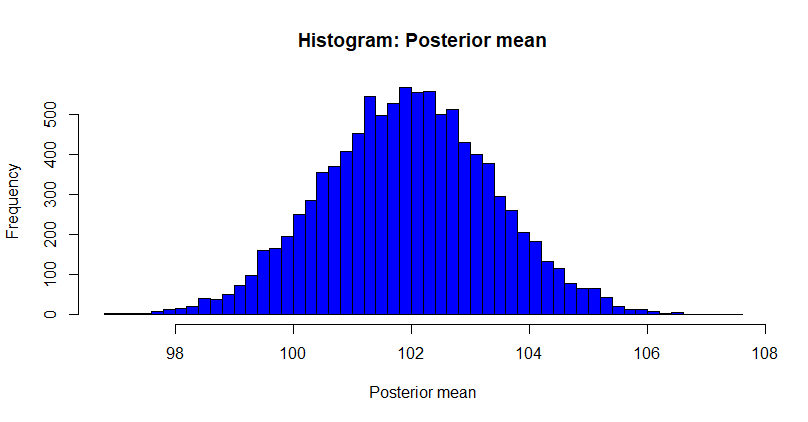
\includegraphics[width=340pt, height=200pt]{Chapters/chapter5/figures/PostMeanMathTest.png}
	%%\centerline{\epsfig{/Chapters/chapter1/figures/cat.eps,width=.8\textheight,height=.4\textwidth}}
	\caption[List of figure caption goes here]{Histogram of posterior draws of mean: Math test}\label{fig51}
\end{figure}

Figure \ref{fig51} shows the histogram of the draws of the posterior mean of the math test results. The posterior mean and median are 101.94 and 101.95, and the 95\% credible interval is (99.14, 104.79).\\

\item Show that the Gibbs sampler is a particular case of the Metropolis-Hastings where the acceptance probability is equal to 1. 

\textbf{Answer}

Without loss of generality let's assume that there are two blocks, $\bm{\theta}=[\bm{\theta}_1 \ \bm{\theta}_2]^{\top}$ such that the Metropolis-Hastings (M-H) algorithm generates a candidate sample $(\bm{\theta}^c_1)$ using a proposal distribution $q(\bm{\theta}^c_1 | \bm{\theta}^{(s-1)})$. The candidate is accepted with probability:
\[
\alpha(\bm{\theta}^{(s-1)}, \bm{\theta}^c) = \min\left\{ 1, \frac{q(\bm{\theta}^{(s-1)}_1 | \bm{\theta}^c) \pi(\bm{\theta}^c | \bm{y})}{q(\bm{\theta}^c_1 | \bm{\theta}^{(s-1)}) \pi(\bm{\theta}^{(s-1)} | \bm{y})} \right\}.
\]

For Gibbs sampling, the candidate $\bm{\theta}^c_1$ is drawn directly from the \emph{full conditional distribution}, so $q(\bm{\theta}^c_1 | \bm{\theta}^{(s-1)}) = \pi(\bm{\theta}^c_1 | \bm{\theta}^{(s-1)}_2, \bm{y})$. Since Gibbs sampling uses the full conditional distributions as the proposal, the key terms simplify. In particular, $q(\bm{\theta}^c_1 | \bm{\theta}^{(s-1)}) = \pi(\bm{\theta}^c_1 | \bm{\theta}^{c}_2, \bm{y})$, and similarly $q(\bm{\theta}^{(s-1)}_1 | \bm{\theta}^c) = \pi(\bm{\theta}^{(s-1)}_1 | \bm{\theta}^{(s-1)}_2, \bm{y})$. Thus, the acceptance probability is given by 
\begin{align*}
	\alpha(\bm{\theta}^{(s-1)}, \bm{\theta}^c) & = \min\left\{ 1, \frac{\pi(\bm{\theta}^{(s-1)}_1 | \bm{\theta}_2^{(s-1)}, \bm{y}) \pi(\bm{\theta}^c | \bm{y})}{\pi(\bm{\theta}^c_1 | \bm{\theta}^{c}_2, \bm{y}) \pi(\bm{\theta}^{(s-1)} | \bm{y})} \right\}\\
	&= \min\left\{ 1, \frac{\pi(\bm{\theta}^{(s-1)}_1 | \bm{\theta}_2^{(s-1)}, \bm{y}) \pi(\bm{\theta}^c_1 | \bm{\theta}^c_2, \bm{y})\pi(\bm{\theta}^c_2 | \bm{y})}{\pi(\bm{\theta}^c_1 | \bm{\theta}^{c}_2, \bm{y}) \pi(\bm{\theta}^{(s-1)}_1 | \bm{\theta}^{(s-1)}_2, \bm{y}) \pi(\bm{\theta}^{(s-1)}_2 | \bm{y})} \right\}\\
	&=1,
\end{align*}
due to $\bm{\theta}^{(s-1)}_2=\bm{\theta}^{c}_2$. Thus, the Gibbs sampling algorithm is implicitly a M-H algorithm where the acceptance probability is 1.

\item Implement a Metropolis-Hastings (M-H) to sample from the Cauchy distribution, $C(0,1)$, using as proposals a standard normal distribution and a Student's t distribution with 5 degrees of freedom. 

\textbf{Answer}

The following code shows to program the M-H to get draws from the Cauchy distribution, $C(0,1)$, using as proposal a standard normal distribution and a Student's t distribution with 5 degree of freedom.

\begin{tcolorbox}[enhanced,width=4.67in,center upper,
	fontupper=\large\bfseries,drop shadow southwest,sharp corners]
	\textit{R code. Metropolis-Hastings algorithm: Cauchy distribution}
	\begin{VF}
		\begin{lstlisting}[language=R]
rm(list = ls()); set.seed(010101)
S <- 100000; df <- 5
theta1 <- runif(S); acept1 <- rep(0, S)
theta2 <- runif(S); acept2 <- rep(0, S)
for (s in 2:S){
	thetac1 <- rnorm(1) # Candidate normal standard
	thetac2 <- rt(1, df = df) # Candidate Students' t
	#Acceptance rate
	a1 <- (dcauchy(thetac1)*dnorm(theta1[s-1]))/(dcauchy(theta1[s-1])*dnorm(thetac1)) 
	a2 <- (dcauchy(thetac2)*dt(theta2[s-1], df = df))/(dcauchy(theta2[s-1])*dt(thetac2, df = df))
	U1 <- runif(1)
	if(U1 <= a1){
		theta1[s] <- thetac1; acept1[s] <- 1
	}else{
		theta1[s] <- theta1[s-1]; acept1[s] <- 0
	}
	if(U1 <= a2){
		theta2[s] <- thetac2; acept2[s] <- 1
	}else{		
		theta2[s] <- theta2[s-1]; acept2[s] <- 0
	}
}
mean(acept1); mean(acept2)
plot(coda::mcmc(theta1)); plot(coda::mcmc(theta2))
h <- hist(theta1, breaks=50, col="blue", xlab="x", main="Cauchy draws from a Metropolis-Hastings algorithm: Normal standard proposal")
pfit <- seq(min(theta1),max(theta1),length=50)
yfit<-dcauchy(pfit)
yfit <- yfit*diff(h$mids[1:2])*length(theta1)
lines(pfit, yfit, col="red", lwd=2)
h <- hist(theta2, breaks=50, col="blue", xlab="x", main="Cauchy draws from a Metropolis-Hastings algorithm: Student's t proposal")
pfit <- seq(min(theta2),max(theta2),length=50)
yfit<-dcauchy(pfit)
yfit <- yfit*diff(h$mids[1:2])*length(theta2)
lines(pfit, yfit, col="red", lwd=2)
\end{lstlisting}
	\end{VF}
\end{tcolorbox} 

Figures \ref{fig52} and \ref{fig53} show the histograms of the posterior draws using the normal and Student's t distributions, along with the density of the Cauchy distribution. The spike in the posterior draws from the standard normal proposal is due to the algorithm being stuck for many iterations at a particular value, as the normal distribution has lighter tails compared to the Cauchy distribution. The convergence using the normal proposal is slower than when using the Student's t proposal, owing to the lighter tails of the former.

\begin{figure}[!h]
	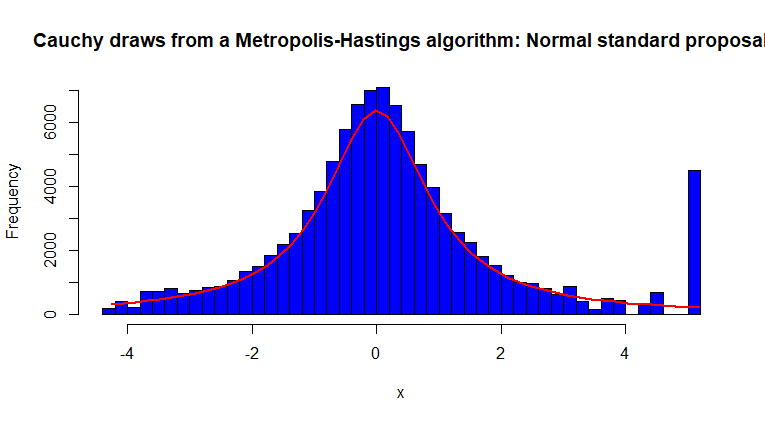
\includegraphics[width=340pt, height=200pt]{Chapters/chapter5/figures/MHnormal.png}
	%%\centerline{\epsfig{/Chapters/chapter1/figures/cat.eps,width=.8\textheight,height=.4\textwidth}}
	\caption[List of figure caption goes here]{Histogram of posterior draws of beta distribution and the density of the beta distribution.}\label{fig52}
\end{figure} 

\begin{figure}[!h]
	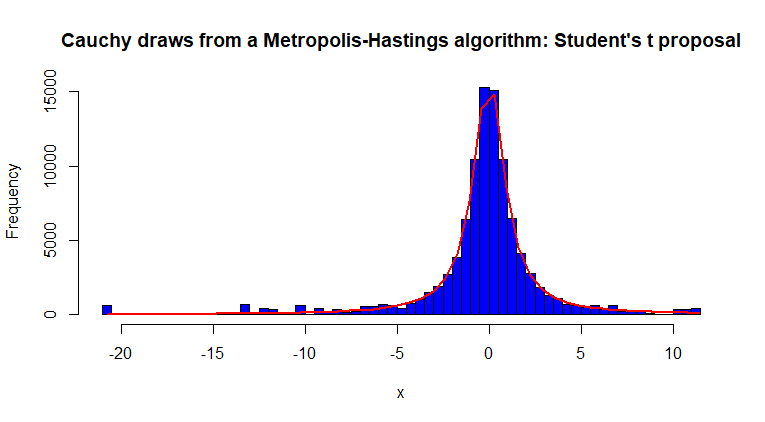
\includegraphics[width=340pt, height=200pt]{Chapters/chapter5/figures/MHt.png}
	%%\centerline{\epsfig{/Chapters/chapter1/figures/cat.eps,width=.8\textheight,height=.4\textwidth}}
	\caption[List of figure caption goes here]{Histogram of posterior draws of beta distribution and the density of the beta distribution.}\label{fig53}
\end{figure} 

\item This exercise was proposed by Professor Hedibert Freitas Lopes, who cites \cite{thomas2021learning} as a useful reference for an introduction to Hamiltonian Monte Carlo in \textbf{R} and the \textit{hmclearn} package. The task is to obtain posterior draws using the Metropolis-Hastings and Hamiltonian Monte Carlo algorithms for the posterior distribution given by 
\[
\pi(\theta_1,\theta_2|\bm{y}) \propto \exp\left\{-\frac{1}{2}(\theta_1^2\theta_2^2 + \theta_1^2 + \theta_2^2 - 8\theta_1 - 8\theta_2)\right\}.
\]
  
  \textbf{Answer}
  
  The following code demonstrates the implementation of the M-H and HMC algorithms for this exercise. For the M-H algorithm, the number of MCMC iterations, burn-in period, and thinning parameters are set to 20,000, 1,000, and 20, respectively. The variance of the proposal distribution is tuned to achieve an acceptance rate close to 25\%. 
  
  For the HMC algorithm, the number of iterations and burn-in period are set to 5,000 and 500, respectively. The step size and number of leapfrog iterations are set to 0.001 and 100, and the mass matrix is defined as \(\bm{M} = \bm{I}_2\). These parameters yield an acceptance rate near 65\%.
  
  Figures \ref{fig54} and \ref{fig55} present the contour plots and posterior draws from the M-H and HMC algorithms for the joint posterior distribution. It can be observed that this distribution is bimodal, and both algorithms successfully capture this feature.
  
 \begin{tcolorbox}[enhanced,width=4.67in,center upper,
 	fontupper=\large\bfseries,drop shadow southwest,sharp corners]
 	\textit{R code. Metropolis-Hastings and Hamiltonian Monte Carlo algorithms}
 	\begin{VF}
 		\begin{lstlisting}[language=R]
rm(list = ls()); set.seed(010101)
# Posterior distribution
PostDist <- function(theta){
	theta1 <- theta[1]; theta2 <- theta[2]
	post <- exp(-0.5*(theta1^2*theta2^2+theta1^2+theta2^2-8*theta1-8*theta2))
	return(post)
}
# Metropolis-Hastings
MH <- function(theta, c2){
	thetac <- MASS::mvrnorm(1, mu = theta, Sigma = c2*diag(2))
	a <- PostDist(thetac)/PostDist(theta)
	U <- runif(1)
	if(U <= a){
		theta <- thetac
		accept <- 1
	}else{
		theta <- theta
		accept <- 0
	}
	return(list(theta = theta, accept = accept))
}
# Posterior draws M-H
S <- 20000; burnin <- 1000; thin <- 20; tot <- S + burnin
K <- 2; c2 <- 1.5
thetaPostMH <- matrix(NA, tot, K)
AcceptMH <- rep(NA, tot)
thetaMH <- c(0, 0)
for(s in 1:tot){
	ResMH <- MH(thetaMH, c2 = c2)
	thetaMH <- ResMH$theta
	thetaPostMH[s,] <- thetaMH
	AcceptMH[s] <- ResMH$accept
}
keep <- seq((burnin), tot, thin)
mean(AcceptMH[keep])
thetaPostMHMCMC <- coda::mcmc(thetaPostMH[keep,])
plot(thetaPostMHMCMC)
coda::autocorr.plot(thetaPostMHMCMC)
# Contour plot
ngrid <- 400
theta1 <- seq(-1, 6, length = ngrid)
theta2 <- seq(-1, 6, length = ngrid)
f <- matrix(0, ngrid, ngrid)
for (i in 1:ngrid){
	for (j in 1:ngrid){
		f[i,j] = PostDist(c(theta1[i],theta2[j]))
	}
}
plot(thetaPostMH[keep,], xlim=range(theta1), ylim=range(theta2), pch=16, col=grey(0.8), xlab=expression(theta[1]), ylab=expression(theta[2]))
contour(theta1,theta2,f, drawlabels=FALSE, add=TRUE, col = "blue", lwd = 1.2)
title("Random walk Metropolis-Hastings")
\end{lstlisting}
 	\end{VF}
 \end{tcolorbox} 

 \begin{tcolorbox}[enhanced,width=4.67in,center upper,
	fontupper=\large\bfseries,drop shadow southwest,sharp corners]
	\textit{R code. Metropolis-Hastings and Hamiltonian Monte Carlo algorithms}
	\begin{VF}
		\begin{lstlisting}[language=R]
HMC <- function(theta, epsilon, L, M){
	Minv <- solve(M); thetat <- theta
	K <- length(thetat)
	mom <- t(mvtnorm::rmvnorm(1, rep(0, K), M))
	logPost_Mom_t <- log(PostDist(thetat)) +  mvtnorm::dmvnorm(t(mom), rep(0, K), M, log = TRUE)  
	theta1 <- theta[1]; theta2 <- theta[2] 
	for(l in 1:L){
		if(l == 1 | l == L){
			mom <- mom + 0.5*epsilon*(-0.5*c(2*theta1*theta2^2+2*theta1-8, 2*theta2*theta1^2+2*theta2-8))
			theta <- theta + epsilon*Minv%*%mom
		}else{
			mom <- mom + epsilon*(-0.5*c(2*theta1*theta2^2+2*theta1-8, 2*theta2*theta1^2+2*theta2-8))
			theta <- theta + epsilon*Minv%*%mom
		}
	}
	logPost_Mom_star <- log(PostDist(theta)) +  mvtnorm::dmvnorm(t(mom), rep(0, K), M, log = TRUE)  
	alpha <- min(1, exp(logPost_Mom_star-logPost_Mom_t))
	u <- runif(1)
	if(u <= alpha){
		thetaNew <- c(theta)
	}else{
		thetaNew <- thetat
	}
	rest <- list(theta = thetaNew, Prob = alpha)
	return(rest)
}
# Posterior draws HMC
S <- 5000; burnin <- 500; tot <- S + burnin
epsilon <- 0.0025;  L <- 100; M <- diag(2)
thetaPostHMC <- matrix(NA, tot, K)
ProbAcceptHMC  <- rep(NA, tot)
thetaHMC <- c(0, 0)
for(s in 1:tot){
	ResHMC <- HMC(theta = thetaHMC, epsilon = epsilon, L = L, M = M)
	thetaHMC <- ResHMC$theta
	thetaPostHMC[s,] <- thetaHMC
	ProbAcceptHMC[s] <- ResHMC$Prob
}
keep <- burnin:S
summary(ProbAcceptHMC[keep])
thetaPostHMCMCMC <- coda::mcmc(thetaPostHMC[keep,])
plot(thetaPostHMCMCMC); coda::autocorr.plot(thetaPostHMCMCMC)
plot(thetaPostHMC[keep,], xlim=range(theta1), ylim=range(theta2), pch=16, col=grey(0.8),
xlab=expression(theta[1]), ylab=expression(theta[2]))
contour(theta1,theta2,f, drawlabels=FALSE, add=TRUE, col = "blue", lwd = 1.2)
title("Hamiltonian Monte Carlo")
\end{lstlisting}
	\end{VF}
\end{tcolorbox} 

 
 \begin{figure}[!h]
 	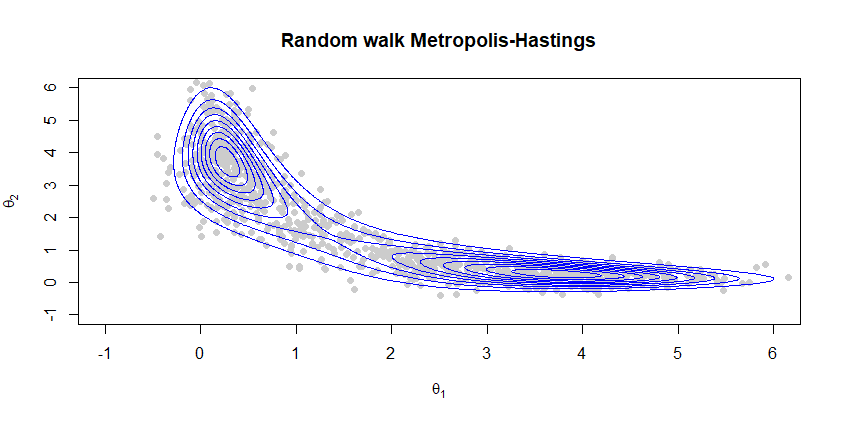
\includegraphics[width=340pt, height=200pt]{Chapters/chapter5/figures/M-Hexample.png}
 	%%\centerline{\epsfig{/Chapters/chapter1/figures/cat.eps,width=.8\textheight,height=.4\textwidth}}
 	\caption[List of figure caption goes here]{Contour plot: Metropolis-Hastings posterior draws.}\label{fig54}
 \end{figure} 
 
 \begin{figure}[!h]
 	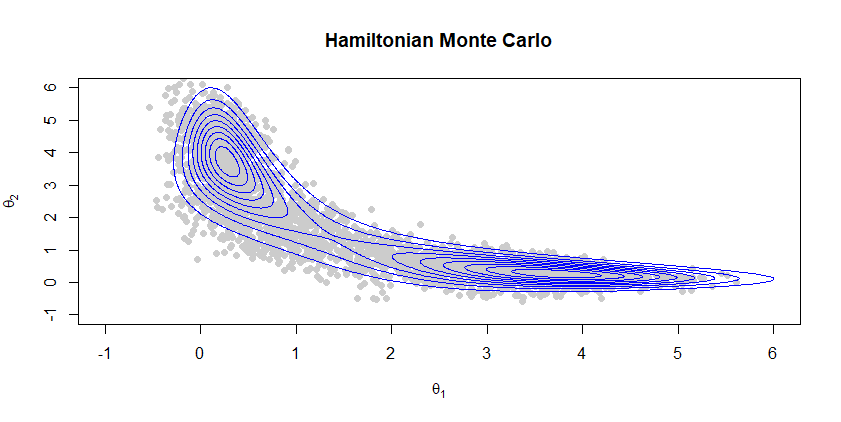
\includegraphics[width=340pt, height=200pt]{Chapters/chapter5/figures/HMCexample1.png}
 	%%\centerline{\epsfig{/Chapters/chapter1/figures/cat.eps,width=.8\textheight,height=.4\textwidth}}
 	\caption[List of figure caption goes here]{Contour plot: Hamiltonian Monte Carlo posterior drwas.}\label{fig55}
 \end{figure} 
 
 \item \textbf{Ph.D. students sleeping hours continues}
 \begin{enumerate}
 	\item Use importance sampling based on a $U(0,1)$ proposal to obtain draws of $\bm{\theta}|\bm{y} \sim B(16.55,39.57)$ in the Ph.D. students' sleeping hours example in Chapter \ref{chap4}. Note that, based on Exercise 15 in Chapter \ref{chap4}, $\alpha_0 = 1.44$ and $\beta_0 = 2.57$.
 	\item Compute the marginal likelihood in this context (Bernoulli-Beta model) and compare it to the result obtained using the Gelfand-Dey method.
 \end{enumerate}

\textbf{Answer}

The posterior distribution of the Bernoulli-beta model is
\begin{align*}
	p(\theta|\bm{y})&=\frac{\prod_{i=1}^N \theta^{y_i}(1-\theta)^{1-y_i}\theta^{\alpha_0-1}(1-\theta)^{\beta_0-1}\Gamma(\alpha_0+\beta_0)}{\Gamma(\alpha_0)\Gamma(\beta_0)p(\bm{y})},
\end{align*}
where 
\begin{align*}
p(\bm{y})&=\int_{\bm{\Theta}}\frac{\prod_{i=1}^N \theta^{y_i}(1-\theta)^{1-y_i}\theta^{\alpha_0-1}(1-\theta)^{\beta_0-1}\Gamma(\alpha_0+\beta_0)}{\Gamma(\alpha_0)\Gamma(\beta_0)}d\theta\\
&=\int_{\bm{\Theta}}\frac{\theta^{\sum _{i=1}^Ny_i+\alpha_0-1}(1-\theta)^{N-\sum_{i=1}^N y_i+\beta_0-1}\Gamma(\alpha_0+\beta_0)}{\Gamma(\alpha_0)\Gamma(\beta_0)}d\theta\\
&=\frac{B(\alpha_n,\beta_n)}{B(\alpha_0,\beta_0)}\int_{\bm{\Theta}}\frac{\theta^{\sum _{i=1}^Ny_i+\alpha_0-1}(1-\theta)^{N-\sum_{i=1}^N y_i+\beta_0-1}}{B(\alpha_n,\beta_n)}d\theta\\
&=\frac{B(\alpha_n,\beta_n)}{B(\alpha_0,\beta_0)}.
\end{align*}
The integral is equal to 1 due to being over the support of $B(\alpha_n,\beta_n)$ distribution.

 \begin{tcolorbox}[enhanced,width=4.67in,center upper,
	fontupper=\large\bfseries,drop shadow southwest,sharp corners]
	\textit{R code. Importance sampling: Bernoulli-Beta model}
	\begin{VF}
		\begin{lstlisting}[language=R]
rm(list = ls()); set.seed(010101); S <- 50000
# Importance sampling from standard normal proposal 
an <- 16.55; bn <- 39.57 # Posterior parameters
theta <- runif(S) # Proposal
ws <- dbeta(theta, an, bn) # Weights
wstars <- ws/sum(ws) # Standardized weights
L <- 20000 # Size of posterior sample
thetaBeta <- sample(theta, L, replace = TRUE, prob = wstars) # Posterior draws
# Figure
h <- hist(thetaBeta, breaks=50, col="blue", xlab="x", main="Beta draws from importance sampling: Uniform (0,1) proposal")
pfit <- seq(min(thetaBeta),max(thetaBeta),length=50)
yfit<-dbeta(pfit, an, bn)
yfit <- yfit*diff(h$mids[1:2])*length(thetaBeta)
lines(pfit, yfit, col="red", lwd=2)
a0 <- 1.44; b0 <- 2.57 # Hyperparameters
s <- 15; n <- 52 # Data
LogMarLik <- lbeta(an, bn)-lbeta(a0, b0) # Marginal likelihood
LogMarLik
# Gelfand-Day method
LikPrior <- function(theta){
	Liki <- theta^s*(1-theta)^(n-s)
	Priori <- dbeta(theta, a0, b0)
	LikPriori <- 1 / Liki * Priori 
	return(LikPriori)
}
LogMarLikGD <- log(1/mean(sapply(thetaBeta, LikPrior)))
LogMarLikGD
\end{lstlisting}
	\end{VF}
\end{tcolorbox} 

Figure \ref{fig55} shows the histogram of the posterior draws obtained using the importance sampling algorithm with a uniform proposal. The algorithm performs well. Additionally, the analytic solution for the log marginal likelihood is -32.75, while the Gelfand-Dey method yields -32.76.

\begin{figure}[!h]
	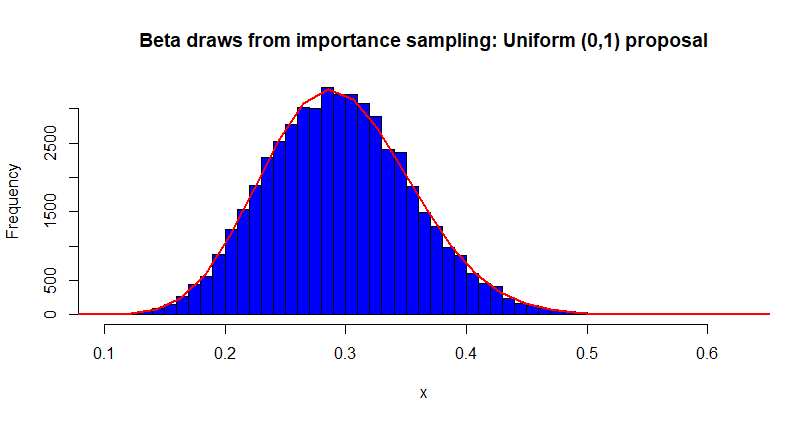
\includegraphics[width=340pt, height=200pt]{Chapters/chapter5/figures/ISbeta.png}
	%%\centerline{\epsfig{/Chapters/chapter1/figures/cat.eps,width=.8\textheight,height=.4\textwidth}}
	\caption[List of figure caption goes here]{Importance sampling: Beta distribution.}\label{fig55}
\end{figure}  
  

\end{enumerate}